\documentclass{beamer}
%~ \documentclass[hyperref={pdfpagelabels=false}]{beamer}

\usepackage[ngerman,english]{babel}
\usepackage[utf8]{inputenc}
\usepackage{lmodern}
\usepackage{beamerthemeshadow}

%\usepackage{la}
\usepackage[T1]{fontenc}

\definecolor{mygreen}{rgb}{0,0.5,0}
\usecolortheme[named=mygreen]{structure}

\usepackage{listings}
\lstdefinestyle{sharpc}{language=[Sharp]C, frame=lr, rulecolor=\color{blue!80!black}}

\title{A Unified Image Processing Framework\\for Computer Vision and Remote Sensing}
\author{
Carsten Brandt,
Ludmilla Brandt,
Marcus Zepp,\\
Akarsh Seggemu
}
\date{May 12, 2015}

\newcommand{\beginbackup}{
   \newcounter{framenumbervorappendix}
   \setcounter{framenumbervorappendix}{\value{framenumber}}
}
\newcommand{\backupend}{
   \addtocounter{framenumbervorappendix}{-\value{framenumber}}
   \addtocounter{framenumber}{\value{framenumbervorappendix}}
}

% table of contents should not show subsections
\setcounter{tocdepth}{1}

% allow using color
\usepackage{color}
\usepackage{xcolor}

% the lstlistings package
\usepackage{listings}
% highlighting lines in listings
\usepackage{linehighlight}

% set colors for code background and highlighting
\definecolor{codehighlight}{rgb}{0.95,0.8,0.8}
\definecolor{codebackground}{rgb}{0.95,0.95,0.95}

%~ % Dadurch wird verhindert, dass die Navigationsleiste angezeigt wird.
%~ \setbeamertemplate{navigation symbols}{}
\setbeamertemplate{footline}{
  \leavevmode%
  \hbox{%
	  \begin{beamercolorbox}[wd=.75\paperwidth,ht=2.25ex,dp=1ex,center]{author in head/foot}%
			\usebeamerfont{author in head/foot}\insertshortauthor%~~(\insertshortinstitute)
	  \end{beamercolorbox}%
%	  \begin{beamercolorbox}[wd=.5\paperwidth,ht=2.25ex,dp=1ex,center]{title in head/foot}%
%			\usebeamerfont{title in head/foot}\insertshorttitle
%	  \end{beamercolorbox}%
	  \begin{beamercolorbox}[wd=.25\paperwidth,ht=2.25ex,dp=1ex,right]{date in head/foot}%
			\usebeamerfont{date in head/foot}\insertshortdate{}\hspace*{2em}
			\insertframenumber{} / \inserttotalframenumber % hier hat's sich geändert
	  \end{beamercolorbox}
	  }%
  \vskip0pt%
}

% http://tex.stackexchange.com/questions/16357/how-can-i-position-an-image-in-an-arbitrary-position-in-beamer
\usepackage{tikz}
%\usetikzlibrary{calc, trees, positioning, arrows, shapes, shapes.multipart, shadows, matrix, decorations.pathreplacing, decorations.pathmorphing}
\usetikzlibrary{arrows}%, shapes, shapes.multipart}

% creating histograms
% http://tex.stackexchange.com/questions/130531/automatic-binning-of-histogram-using-raw-gnuplot-in-pgfplot
% \usepackage{pgfplots}
% \usepackage{pgfplotstable}
% \usetikzlibrary{external}
% \tikzexternalize
% \tikzset{external/force remake}
% %\pgfplotsset{compat=1.8}


\tikzset{
  every boverlay node/.style={
    draw=black,fill=white,rounded corners,anchor=north west,
  },
}
\tikzset{
  every overlay node/.style={
    %draw=white,fill=white,rounded corners,anchor=north west,
    anchor=north west
  },
}
% Usage:
% \tikzoverlay at (-1cm,-5cm) {content};
% or
% \tikzoverlay[text width=5cm] at (-1cm,-5cm) {content};
\def\tikzboverlay{%
   \tikz[baseline,overlay]\node[every boverlay node]
}%
\def\tikzoverlay{%
   \tikz[baseline,overlay]\node[every overlay node]
}%

\usetheme{default}
% default, bars, boxes, classic, lined, plain, shadow, sidebar, split, tree
% Berlin, Darmstadt, Dresden, Frankfurt, Goettingen, Hannover, Ilmenau, Luebeck, . . . , Warsaw

\usepackage{pdfpcnotes}

% Notizen zu jeder Folie auf zweitem Bildschirm anzeigen
%~ \setbeameroption{show notes on second screen = right}
% Notizen beliebig innerhalb des Frames setzen:
% 1 (...)
% 2 \note{Hier eine Notiz}
% 3 (...)
% 4 \note[item]{und noch eine Notiz , diesmal geordnet}
% 5 (...)



\definecolor{codehighlight}{rgb}{0.95,0.8,0.8}
\definecolor{codebackground}{rgb}{0.95,0.95,0.95}

\definecolor{exercisecolor}{rgb}{0.63, 0.90, 1.00}

\definecolor{lightgrey}{rgb}{0.9,0.9,0.9}
\definecolor{mygreen}{rgb}{0,0.6,0}
\definecolor{mygray}{rgb}{0.5,0.5,0.5}
\definecolor{mymauve}{rgb}{0.58,0,0.82}

\lstset{ %
%	backgroundcolor=\color{lightgrey},   % choose the background color; you must add \usepackage{color} or \usepackage{xcolor}
	breakatwhitespace=true,          % sets if automatic breaks should only happen at whitespace
	breaklines=true,                 % sets automatic line breaking
	captionpos=b,                    % sets the caption-position to bottom
%	deletekeywords={...},            % if you want to delete keywords from the given language
%	escapeinside={\%*}{*)},          % if you want to add LaTeX within your code
%	extendedchars=true,              % lets you use non-ASCII characters; for 8-bits encodings only, does not work with UTF-8
	frame=single,                    % adds a frame around the code
	keepspaces=true,                 % keeps spaces in text, useful for keeping indentation of code (possibly needs columns=flexible)
	language=C++,                    % the language of the code
	morekeywords={*,php,class,extends,public,protected,private,foreach,if,else,elseif,%
		function,return,new,echo,endforeach,vector,Context
	},            % if you want to add more keywords to the set
	numbers=left,                    % where to put the line-numbers; possible values are (none, left, right)
	numbersep=10pt,                   % how far the line-numbers are from the code
%	rulecolor=\color{black},         % if not set, the frame-color may be changed on line-breaks within not-black text (e.g. comments (green here))
	showspaces=false,                % show spaces everywhere adding particular underscores; it overrides 'showstringspaces'
	showstringspaces=false,          % underline spaces within strings only
	showtabs=false,                  % show tabs within strings adding particular underscores
	stepnumber=1,                    % the step between two line-numbers. If it's 1, each line will be numbered
	tabsize=4,                       % sets default tabsize to 2 spaces
%	title=\lstname                   % show the filename of files included with \lstinputlisting; also try caption instead of title
	basicstyle=\footnotesize\ttfamily,
	keywordstyle=\bfseries\color{green!40!black},
	commentstyle=\color{purple!40!black},
	identifierstyle=\color{black},
	stringstyle=\color{orange},
	numberstyle=\tiny\color{mygray}, % the style that is used for the line-numbers
}

%  \beamersetuncovermixins{\opaqueness<1>{25}}{\opaqueness<2->{15}}
%  sorgt dafuer das die Elemente die erst noch (zukuenftig) kommen
%  nur schwach angedeutet erscheinen
\beamersetuncovermixins{\opaqueness<1>{25}}{\opaqueness<2->{15}}
% klappt auch bei Tabellen, wenn teTeX verwendet wird\ldots

\begin{document}


\begin{frame}
	\titlepage
\end{frame}

\begin{frame}
	\tableofcontents  \pnote{}
\end{frame}

% Vor jedem Abschnitt automatisch Inhaltsverzeichnis anzeigen:
\AtBeginSection []{
\begin{frame}
	\tableofcontents [currentsection]

	\pnote{
		notes go here...
	}
\end{frame}
}

%---------------------------------------------------------------------------------------------------------------------------------------------
\section{What is this all about?}
\begin{frame}{Unified Image Processing Framework}


	\includegraphics<1>[width=\textwidth]{images/intro/simpleChain}
	\includegraphics<2>[width=.9\textwidth]{images/intro/complexChain}

	\pnote{
		Framework which allows you to divide your program in many steps,
		which can be combined in arbitrary ways, and also gives you the
		possibility to store each of your chains, with all inputs and params.
	}

\end{frame}

\begin{frame}{Reasons to use}

%	\begin{itemize}
%	\end{itemize}

	\pnote{
		- easy to use \\
		- extensible \\
		- visualization of steps \\

		- better reuse of modules \\
		- allows sharing modules \\

		- practical storage of chains with different inputs \\

		- "platform independent" \\
		- "parallel execution of steps" \\
	}

\end{frame}


\section{Working with the program}
\subsection{User Interfaces}
\begin{frame}[t]{User Interfaces}

	\begin{columns}
		\begin{column}[t]{.5\textwidth}
			\begin{center}
			{\Large GUI}
			\vspace{.5cm}

			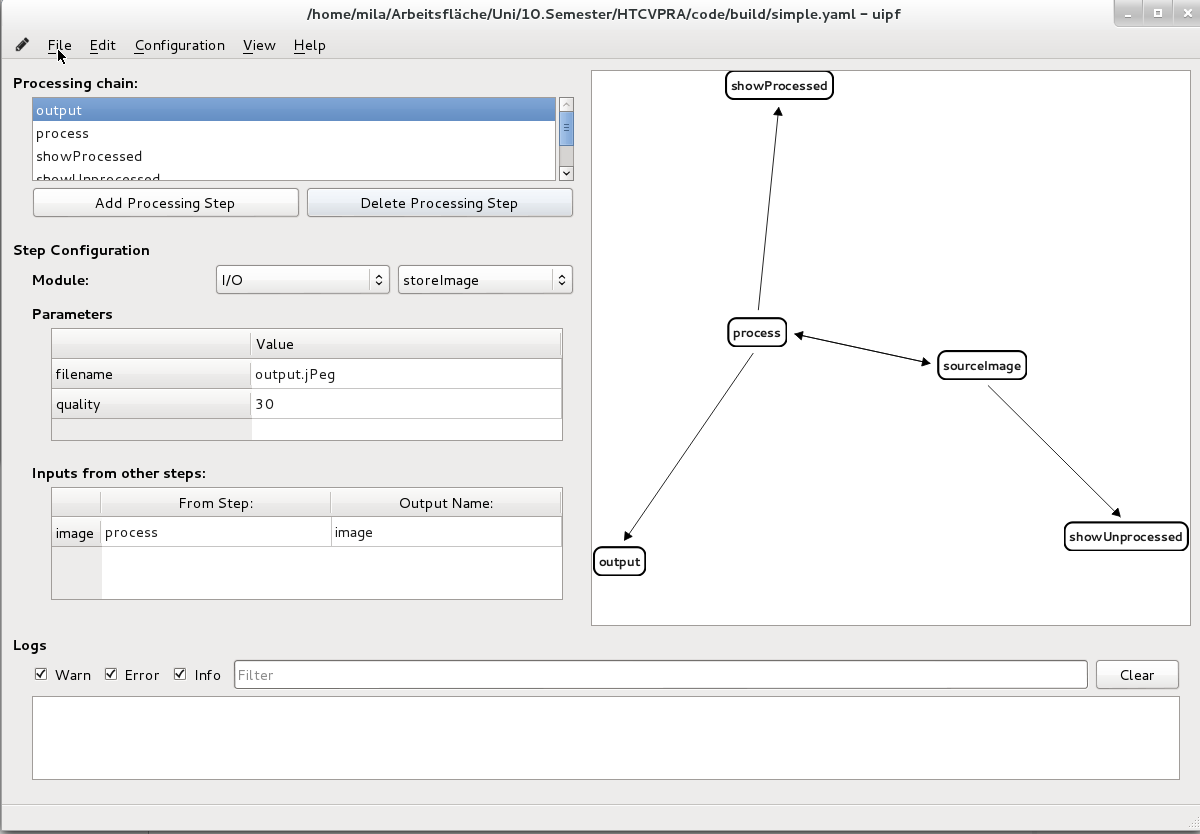
\includegraphics[width=\textwidth]{images/howto/gui}

			\end{center}
		\end{column}
		\begin{column}[t]{.5\textwidth}
			\begin{center}
			{\Large Console}
			\vspace{.5cm}

			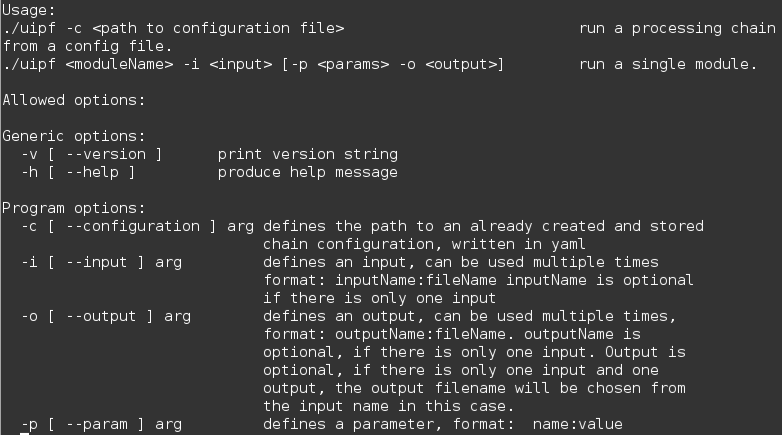
\includegraphics[width=\textwidth]{images/howto/console}

			\end{center}
		\end{column}
	\end{columns}

	\pnote{
		framework provides two interfaces: GUI, Console

		these share a common file format in YAML.

		GUI can create and run chains.

		Console can run a chain and also run single modules.
	}

\end{frame}

\subsection{General Concepts}
\begin{frame}{General Concepts}

	\begin{columns}
		\begin{column}[t]{.4\textwidth}
\Large
			Processing Chain
			\vspace{.4cm}\pause
\Large
			\begin{itemize}
				\item[$\rightarrow$] Processing Step
				\vspace{.25cm}\pause
				\large
				\begin{itemize}
					\item[$\rightarrow$] Module
				\vspace{.25cm}\pause
					\item[$\rightarrow$] Parameters
				\vspace{.25cm}\pause
					\item[$\rightarrow$] Dependencies
				\end{itemize}
			\end{itemize}

		\end{column}
		\begin{column}[t]{.6\textwidth}
			\begin{center}

				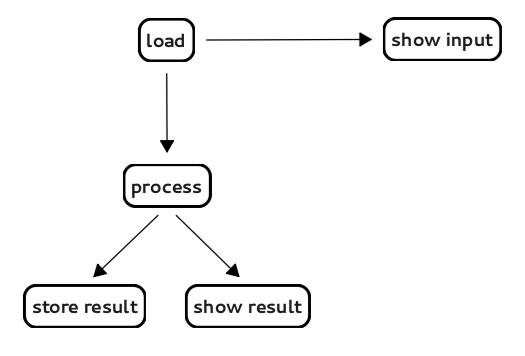
\includegraphics[width=\textwidth]{images/intro/simpleChain}

			\end{center}
		\end{column}
	\end{columns}

\end{frame}

\begin{frame}{General Concepts}

	\includegraphics<1>[width=\textwidth]{images/existingChain}
	\includegraphics<2>[width=\textwidth]{images/runChain}
	\includegraphics<3>[width=\textwidth]{images/stopChain}
	\includegraphics<4>[width=\textwidth]{images/newChain}
	\includegraphics<5>[height=\textheight]{images/buggyChain}


	\pnote{
		open an existing chain\\
		run/stop the chain\\
		create a new chain/modify existing chain\\
		save the chain\\
		run a buggy chain
	}

\end{frame}



\subsection{Console}
\begin{frame}{How to use}

	\includegraphics<1>[width=\textwidth]{images/ConsoleHelp}
	\includegraphics<2>[width=\textwidth]{images/ConsoleYaml}
	\includegraphics<3>[width=\textwidth]{images/ConsoleShort}


	\pnote{
		how to use help\\
		how to run a chain\\
		how to run a single module\\
	}

\end{frame}


\subsection{How to create a new chain by hand}
\begin{frame}[fragile]{How to use}

	\begin{lstlisting}
conv:
  module: convolution
  input:
    image: gaus.image
    kernel: load.image
  anchorX: ""
  anchorY: ""
  delta: ""
gaus:
  module: gaussian
  input:
    image: load.image
  sigmaX: 3
  sigmaY: 3
  windowSize: ""
load:
  module: loadImage
  filename: hier.png
  mode: ""
show:
  module: showImage
  input:
    image: gaus.image
  blocking: ""
  title: ""
	\end{lstlisting}


	\pnote{
		human readyble\\
		uses keywords and indentations
	}

\end{frame}

\section{How to write a new module}

\subsection{What is a module}
\begin{frame}[fragile]{Idea}

	Basic interface:
	\begin{lstlisting}
		void run(DataManager& data)
		string name()
		MetaData getMetaData()
	\end{lstlisting}

 	MataData:
	\begin{lstlisting}
		string, // general verbal description of the module
		string, // category
		map<string, DataDescription>, // input
		map<string, DataDescription>, // output
		map<string, ParamDescription> // params
	\end{lstlisting}


	\pnote{
		A method
	}

\end{frame}


\begin{frame}[fragile]{run() method}

	\begin{lstlisting}<1>
void LoadImageModule::run( DataManager& data) const
{
	// (1) get inputs and params:
	//     - data.getInputData(inputName)
	//     - data.getParam (paramName, dafaultValue)
	// (2) work with them
	// (3) create output:
	//     - data.setOutputData(outputName, outputContent);
}
	\end{lstlisting}

\end{frame}


\begin{frame}[fragile]{getMetaData() method}

\begin{linehighlight}{
%      \only<1,3>{ % Only on slides 1 and 3 (beamer stuff)
%            \highline{1,3,5} % highlight code lines 1,3 and 5.
%      }
%      \only<2>{ % Only on slide 2 (beamer)
%            \highline{2,...,8} % highlight lines 2 to 8.
%      }
}
      \lstinputlisting{metadata.cpp}
\end{linehighlight}

\end{frame}


\section{Testing}
\begin{frame}{run with TestRail}
	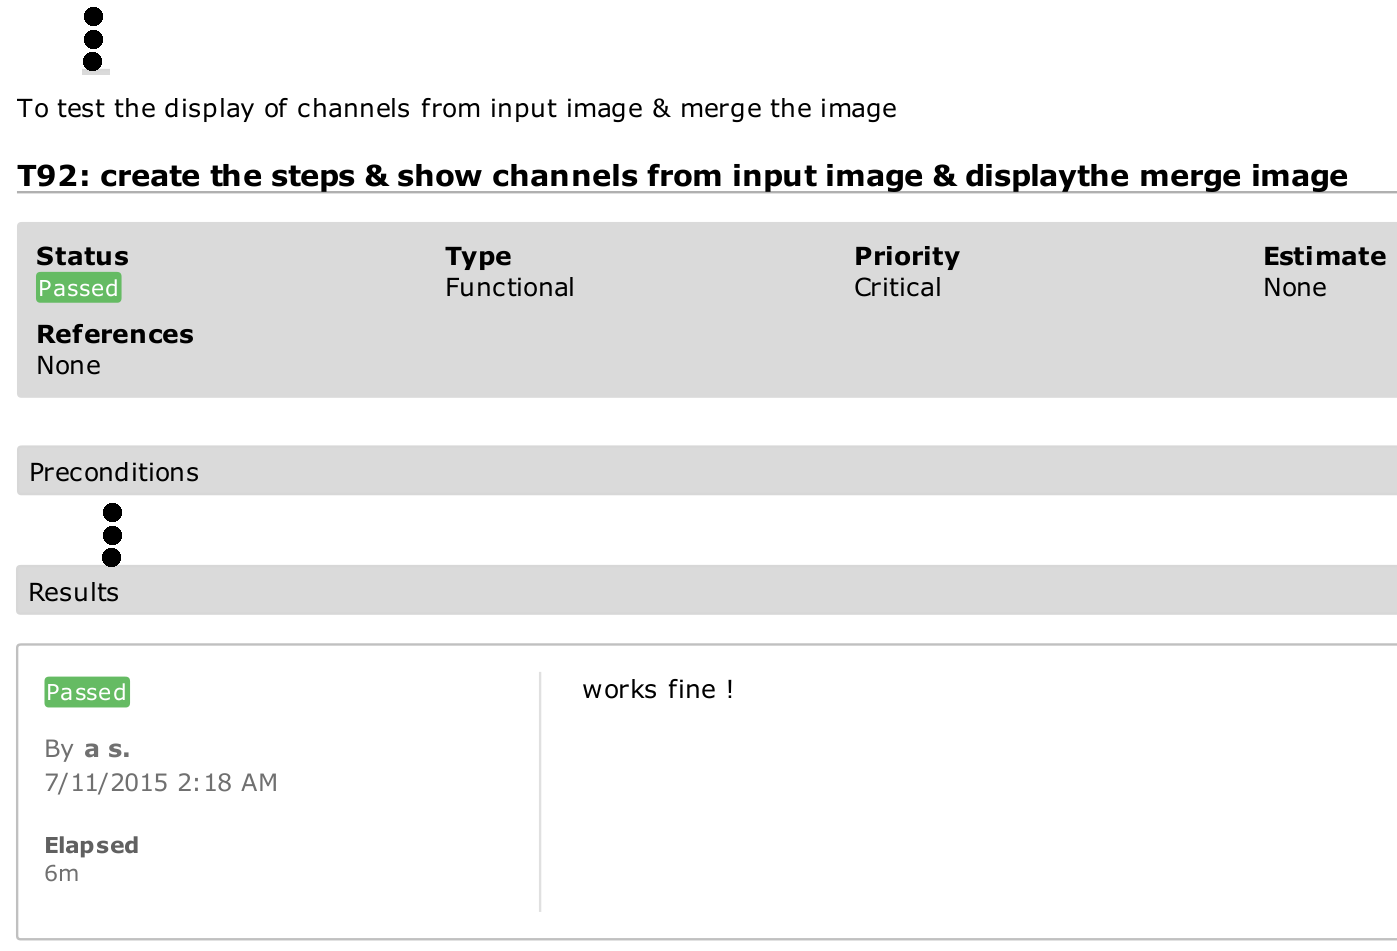
\includegraphics[width=\textwidth]{images/eval}
\end{frame}

\begin{frame}{Video Tutorial}
	%~ \includegraphics[width=\textwidth]{images/tutorial}
\end{frame}

\section{Live Demo}

\begin{frame}{Live Demo}

\begin{center}
	{\Huge
	Live Demo!}
	\vspace{2cm}

	Fork us on Github:\\\vspace{0.2cm}
	\url{https://github.com/TU-Berlin-CVRS/uipf}

	\pnote{
		first: Questions?\\
		We are on github!\\
		second: Live Demo.
	}
\end{center}
\end{frame}


%\beginbackup
%\section{Appendix}

%\begin{frame}
%	\frametitle{Pack-Man}
%...
%\end{frame}

%\backupend

\end{document}
